%% LaTeX-Beamer template for KIT design
%% by Erik Burger, Christian Hammer
%% title picture by Klaus Krogmann
%%
%% version 2.1
%%
%% mostly compatible to KIT corporate design v2.0
%% http://intranet.kit.edu/gestaltungsrichtlinien.php
%%
%% Problems, bugs and comments to
%% burger@kit.edu

\documentclass[18pt]{beamer}
\usepackage[utf8x]{inputenc}
\usepackage{units}
\usepackage{booktabs}

%% CUSTOM
\usepackage{amsmath}
\usepackage{algpseudocode}
%\usepackage{kbordermatrix}
%% GBI-Stuff
% \usepackage{tikz}
%\usetikzlibrary{arrows,shapes}
%\usetikzlibrary{automata}
%\usetikzlibrary{matrix}

%% Definitions
\DeclareMathOperator{\div2}{div}
\renewcommand{\algorithmicrequire}{\textbf{Input:}}
\renewcommand{\algorithmicensure}{\textbf{Output:}}
\newcommand{\sq}{$\square$}
\newcommand{\da}{$\downarrow$}
\algnewcommand\algorithmicto{\textbf{to}}
\algrenewtext{For}[3]{\algorithmicfor\ $#1 \gets #2$ \algorithmicto\ $#3$ \algorithmicdo}
%\algrenewtext{If}[1]{\alggorithmicdo}
%\algrenewtext{EndIf}{\algorithmicod}
\algnewcommand\algorithmicod{\textbf{od}}
\algrenewtext{EndWhile}{\algorithmicod}
\algrenewtext{EndFor}{\algorithmicod}
\AtBeginSection[]{%
\begin{frame}<beamer> % do nothing in handouts
    \frametitle{Überblick}
    \tableofcontents[sectionstyle=show/shaded,
    subsectionstyle=show/show/hide]
\end{frame}
}
%\AtBeginSubsection[]{%
%\begin{frame}<beamer> % do nothing in handouts
%    \frametitle{Überblick}
%    \tableofcontents[sectionstyle=show/shaded,
%    subsectionstyle=show/shaded/hide]
%\end{frame}
%}

%% SLIDE FORMAT

% use 'beamerthemekit' for standard 4:3 ratio
% for widescreen slides (16:9), use 'beamerthemekitwide'

\usepackage{templates/beamerthemekit}
%\usepackage{templates/beamerthemekitwide}

 %% TITLE PICTURE

 % if a custom picture is to be used on the title page, copy it into the 'logos'
 % directory, in the line below, replace 'mypicture' with the 
 % filename (without extension) and uncomment the following line
 % (picture proportions: 63 : 20 for standard, 169 : 40 for wide
 % *.eps format if you use latex+dvips+ps2pdf, 
 % *.jpg/*.png/*.pdf if you use pdflatex)


\titleimage{banner}
 
 
%% Define some colors:
\definecolor{darkblue}{rgb}{0,0,.5}
\definecolor{darkgreen}{rgb}{0,.5,0}

 %% TITLE LOGO

 % for a custom logo on the front page, copy your file into the 'logos'
 % directory, insert the filename in the line below and uncomment it

\titlelogo{empty_logo}
 
 % (*.eps format if you use latex+dvips+ps2pdf,
 % *.jpg/*.png/*.pdf if you use pdflatex)
 
 %% TikZ INTEGRATION
 
 % use these packages for PCM symbols and UML classes
 % \usepackage{templates/tikzkit}
 % \usepackage{templates/tikzuml}
 
 % the presentation starts here
 
\author{Lukas B\"ohm, Lukas Feller, Marcel Kost, Nicholas Kj\"ar}
\institute{Institut f\"ur Informatik}

\setbeamertemplate{caption}{\raggedright\insertcaption\par}


\title[LLNM]{LLNM - Zwischenpräsentation}
\subtitle{}
\date{\today}
\begin{document}
	%title page
	\begin{frame}
		\titlepage
	\end{frame}
	\begin{frame}{Benchmarking: Cube.json}
		\begin{tabular}{l*{4}{r}}
		Methode           & Preprocessing & Rendering & Render Speedup \\%& Total  \\
		\hline
		rein sequentiell  & /      & 5837ms & /      \\%& 6847ms \\
		OpenMP            & /      & 3023ms & 1.93   \\%& 5022ms \\
		BiH               & 0.3ms  & 1452ms & 4.02   \\%& 2592ms \\
		SSE               & /      & 2079ms & 2.81   \\%& 3537ms \\
		Subsampling       & /      & 3374ms & 1.73   \\%& 4711ms \\
		OpenMP + BiH      & 0.3ms  &  904ms & 6.45   \\%& 2354ms \\
		OpenMP + SSE      & /      &  901ms & 6.48   \\%& 2724ms \\
		\end{tabular}
	\end{frame}
	\begin{frame}{Benchmarking: Sponza.json}
		\begin{tabular}{l*{4}{r}}
		Methode           & Preprocessing & Rendering & Render Speedup \\%& Total  \\
		\hline
		rein sequentiell  & /      & $>$10min & /        \\
		OpenMP + BiH      & 39ms   & 41.3s    & $>$ 14.5 \\
		OpenMP + BiH + Sub  & 39ms   & 21.0s    & $>$ 29 \\
		OpenMP + SSE      & /      & 150s     & $>$ 4    \\
		\end{tabular}
	\end{frame}
	\begin{frame}{BIH Datenstruktur}
		\begin{figure}[ht]
		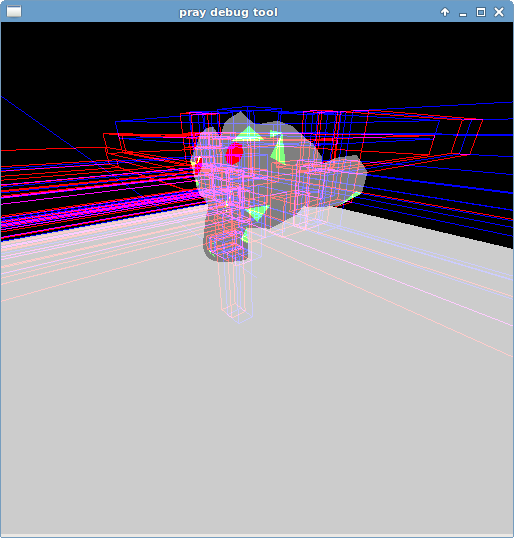
\includegraphics[height=0.8\textheight]{images/bih2.png}
		\end{figure}
	\end{frame}

	\begin{frame}{Abweichung vom Beispielbild}
		\center
		
\includegraphics[height=0.8\textheight]{images/cropped_diff_ref.png}
	\end{frame}
	\begin{frame}{Abweichung mit schnellerem Runden}
		\center
		
\includegraphics[height=0.8\textheight]{images/cropped_diff_round.png}
	\end{frame}
	\begin{frame}{Abweichung mit -Ofast}
		\center
		
\includegraphics[height=0.8\textheight]{images/cropped_diff_fast.png}
	\end{frame}
	\begin{frame}{Abweichung mit Subsampling}
		\center
		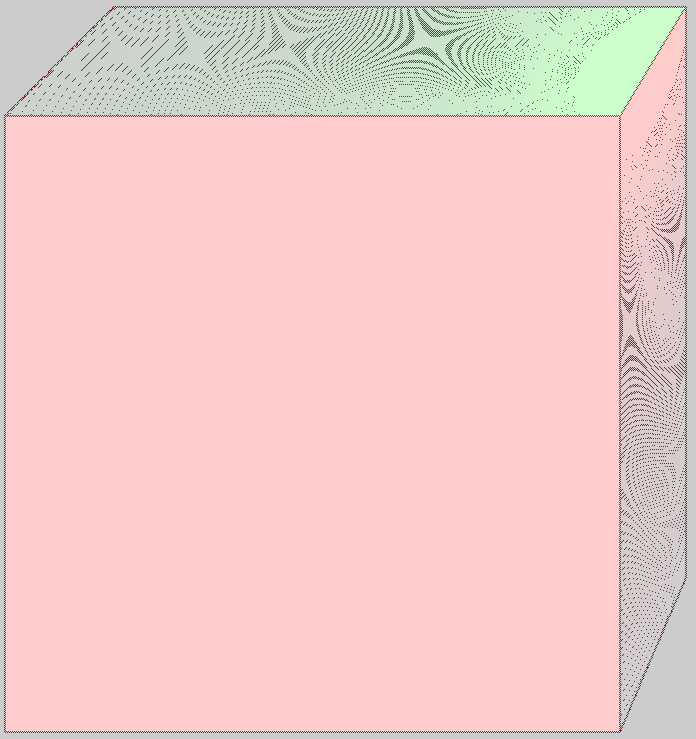
\includegraphics[height=0.8\textheight]{images/cropped_diff_ss.png}
	\end{frame}

	\begin{frame}{Hot Code Paths}
		\begin{figure}[ht]
			\begin{columns}
				\begin{column}{.48\textwidth}
					\center
					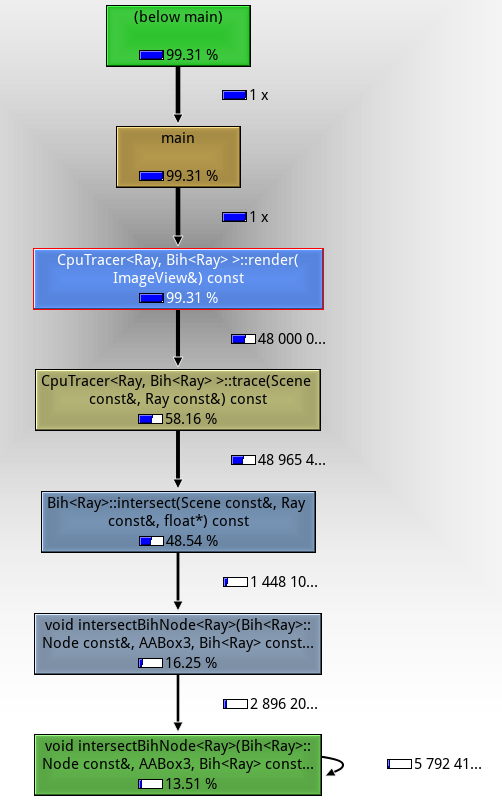
\includegraphics[height=.7\textheight]{images/callgrind_bih.png}
					\caption{KCachegrind-Graph für pray mit BIH}
				\end{column}
				\begin{column}{.48\textwidth}
					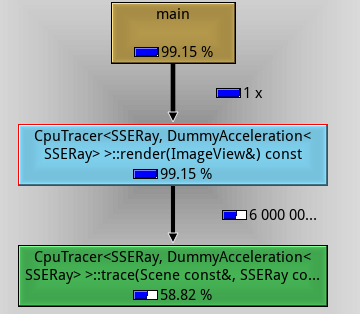
\includegraphics[width=\textwidth]{images/callgrind_sse.png}
					\caption{KCachegrind-Graph für pray mit SSE}
				\end{column}
			\end{columns}
	\end{figure}
	\end{frame}

	\begin{frame}{Ausblick}
		\begin{figure}[ht]
		\vspace{1cm}
		\begin{minipage}{0.45\linewidth}
			\begin{itemize}
				\item Cuda
				\item SSE + BIH verheiraten
				\item Andere Beschleunigungsstrukturen
			\end{itemize}
			\vspace{4.5cm}
		\end{minipage}
		\begin{minipage}[b]{0.45\linewidth}
			\centering
			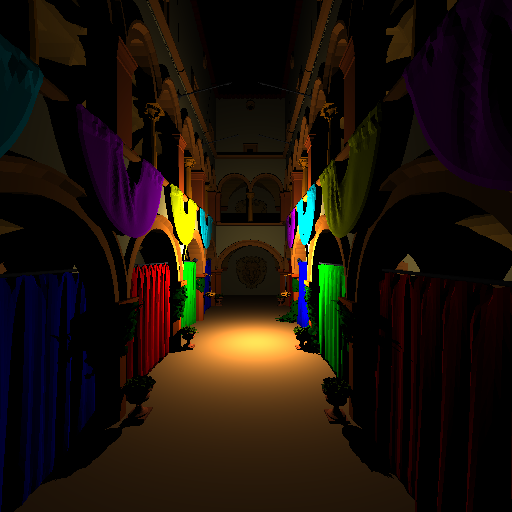
\includegraphics[width=\textwidth]{images/sponza.png}
		\end{minipage}
	\end{figure}
		
	\end{frame}
\end{document}
